%%%%%%%%%%%%%%%%%%%%%%%%%%%%%%%%%%%%%%%%%
% Short Sectioned Assignment
% LaTeX Template
% Version 1.0 (5/5/12)
%
% This template has been downloaded from:
% http://www.LaTeXTemplates.com
%
% Original author:
% Frits Wenneker (http://www.howtotex.com)
%
% License:
% CC BY-NC-SA 3.0 (http://creativecommons.org/licenses/by-nc-sa/3.0/)
%
%%%%%%%%%%%%%%%%%%%%%%%%%%%%%%%%%%%%%%%%%

%----------------------------------------------------------------------------------------
%   PACKAGES AND OTHER DOCUMENT CONFIGURATIONS
%----------------------------------------------------------------------------------------

\documentclass[11pt, oneside]{article} % A4 paper and 11pt font size
\usepackage[margin=1in]{geometry}
\geometry{letterpaper}

\usepackage{pslatex}
\usepackage[T1]{fontenc} % Use 8-bit encoding that has 256 glyphs
\usepackage[english]{babel} % English language/hyphenation
\usepackage{amsmath,amsfonts,amsthm} % Math packages

\usepackage{lipsum} % Used for inserting dummy 'Lorem ipsum' text into the template

\usepackage{graphicx} % Required for including pictures
\usepackage{wrapfig}
\usepackage{caption}
\usepackage{subcaption}
\usepackage{float}
\usepackage{enumitem}
\usepackage{listings}
\usepackage{color}
\usepackage[]{hyperref}


\usepackage{sectsty} % Allows customizing section commands

\numberwithin{equation}{section} % Number equations within sections (i.e. 1.1, 1.2, 2.1, 2.2 instead of 1, 2, 3, 4)
\numberwithin{figure}{section} % Number figures within sections (i.e. 1.1, 1.2, 2.1, 2.2 instead of 1, 2, 3, 4)
\numberwithin{table}{section} % Number tables within sections (i.e. 1.1, 1.2, 2.1, 2.2 instead of 1, 2, 3, 4)

%\setlength\parindent{0pt} % Removes all indentation from paragraphs - comment this line for an assignment with lots of text

\renewcommand{\c}[1]{\texttt{#1}}
\newcommand\todo[1]{\textbf{\textcolor{red}{#1}}}
\newcommand{\teambb}{\c{bennyblum }}
\newcommand{\teamol}{\c{louisofir }}
\DeclareMathOperator{\MD}{MD}

%----------------------------------------------------------------------------------------
%   TITLE SECTION
%----------------------------------------------------------------------------------------

\title{ 
Tweetnet: Finding the bots of the flock\
}

\author{
Josh Blum (joshblum@mit.edu)\\
Bennet Cyphers (bcyphers@mit.edu)\\
Ofir Nachum (ofir@mit.edu)\\
Louis Sobel (sobel@mit.edu)\\
\\
6.857 Final Project
\date{\today}
}

\begin{document}

\maketitle

\vfill

\begin{abstract}
\todo{blah blah black sheep}
\end{abstract}

\clearpage

\section {Introduction}

\section {Related Work}
Botnets using social networks for command and control are a relatively recent phenomenon. These botnets take advantage of the reliable infrastructure and easy-to-use APIs of social networks to communicate commands to infected computers. Several of these botnets have already been detected. 

Several botnets have been discovered in the wild \cite{arbor, trendmicro, flashback}. In 2009, Arbor Networks \cite{arbor} discovered a Twitter bot which periodically tweets base-64 encoded commands that specify URLs for downloading malicious binaries. The Mehika botnet \cite{trendmicro} is another botnet which was found utilizing Twitter to send commands to its botslaves. The Macintosh Flashware malware provides another example of a botnet using Twitter for command and control \cite{flashback}. The malware queries Twitter for tweets containing specific hashtags. 

In addition to these detected botnets, several groups have designed and implemented social networking botnets \cite{socialnetworking, trojan7, stegobot}. A group of San Jose University researchers design and implement their \emph{SocialNetworkingBot} to issue commands via Twitter for such things as browsing a URL, taking a screenshot, shutting down the computer, or changing botmaster \cite{socialnetworking}. Another notable example is a group of researches developing \emph{Stegobot}, a botnet which covertly communicates via JPEG stegonography of images shared on social networks. These examples highlight the ease in which it is possible to use social networks as botnet infrastructure.

In response the the growing threat of botnets using social networks, researchers have proposed several detection mechanisms to thwart such botnets \cite{botsniffer, kartaltepe, burghouwt}. Gu et al. propose an approach using network-based anomaly detection \cite{botsniffer}. These methods are useful when botnet activity is temporally correlated. Kartaltepe et al. present a content-specific method, proposing a classifier for classifying natural text from base-64 or otherwise encoded commands \cite{kartaltepe}. The group also suggests client-side detection mechanisms that are alerted by network traffic of dubious origin (for example, if a Twitter URL is requested when no browser actually has Twitter displayed).

The previous work in this field shows that, while botnets using social networks is a relatively recent phenomenon, the threat of even better concealed botnets is growing rapidly. For this reason, it is imperative that new detection mechanisms be devised.

\section{Game Overview}
	\subsection{Justification}
	\subsection{Infrastructure}
	\subsection{Rules}

% \section{Meet the Team}
% 	\subsection{Team Blumbenny}

% 	\begin{figure}
% 		\centering
% 		\begin{subfigure}{.4\textwidth}
% 			\centering
% 			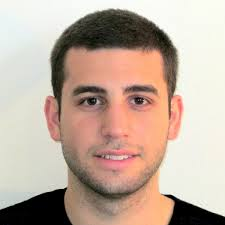
\includegraphics[width=.4\textwidth]{resources/blum.jpg}
% 			\caption{Blum}
% 		\end{subfigure}
% 		\begin{subfigure}{.4\textwidth}
% 			\centering
% 			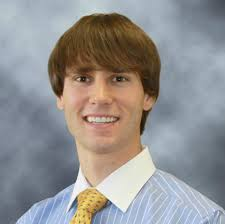
\includegraphics[width=.4\textwidth]{resources/benny.jpg}
% 			\caption{Benny}
% 		\end{subfigure}
% 		\caption{Team Blumbenny}
% 	\end{figure}


% 	\subsection{Team Lofir}
	
% 		\begin{figure}
% 		\centering
% 		\begin{subfigure}{.4\textwidth}
% 			\centering
% 			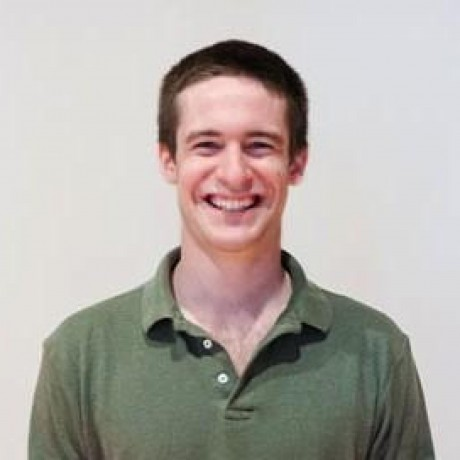
\includegraphics[width=.4\textwidth]{resources/louis.jpg}
% 			\caption{Louis}
% 		\end{subfigure}
% 		\begin{subfigure}{.4\textwidth}
% 			\centering
% 			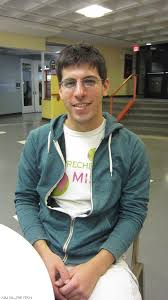
\includegraphics[width=.4\textwidth]{resources/ofir.jpg}
% 			\caption{Ofir}
% 		\end{subfigure}
% 		\caption{Team Lofir}
% 	\end{figure}

\section{Round 1}
	\subsection{Setup}
		During the first round, each team designed a single \c{Bot} and \c{BotMaster} pair which had to submit a single flag. There were 10 unique handles used in the game pool, of which 1 was the botmaster and the other 9 being benign users, which would tweet with a $0.20$ probability each second. \teambb's bots knew the botmaster handle at the beginning of the round whereas \teamol's bots established the botmaster as part of their design. \\

		In this round bots were allowed to begin arbitrary secrets such as values for a random seed or cryptographic keys. The goal of this round was to allow the teams to familiarize themselves with the game infrastructure and begin building discovery techniques. For this reason, we allowed may simplifications to the game structure for this round, with the intent of modifying the game structure in the subsequent round. 

	\subsection{Designs}
		\subsubsection{\teambb}
			\teambb built the \c{SingelCharBotMaster} which relied on a \c{prng} to signify tweets which were information carrying. The botmaster and bots both shared a common seed value for the \c{prng}. The \c{prng} was also used to transfer a single character in each tweet that was information carrying. The character offset and value for which information tweets was used by each next random value. Figure \ref{fig:prng} shows an example of how the \c{prng} was used to offset information tweets, and figure \ref{fig:prng-tweet-ex} shows how this offset is used to store a character of the flag within a tweet. \\

		\begin{figure}[H]
		    \center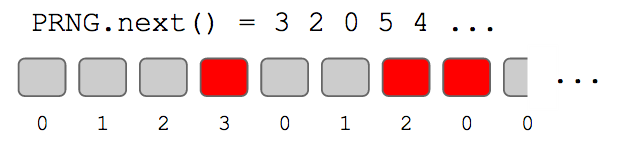
\includegraphics[scale=0.70]{resources/prng.png}
		    \caption{An example of how the \c{SingleCharBotMaster} design uses a \c{prng} to offset which tweets carry information.}
		    \label{fig:prng}
		 \end{figure}

		 \begin{figure}[H]
		    \center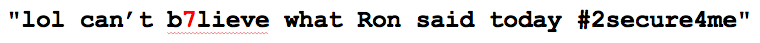
\includegraphics[scale=0.60]{resources/prng-tweet-ex.png}
		    \caption{An example of how the \c{SingleCharBotMaster} design stores flag information in a information carrying tweet.}
		    \label{fig:prng-tweet-ex}
		 \end{figure}
		
			
		\subsubsection{\teamol}
			\teamol built the \c{SpaceBotmaster}. This botmaster used a space at the end of tweet text to signify a flag-relevant tweet. The master would insert a punctuation mark immediately preceding the space (`.', `,', `!', `?'), and this would provide two bits of the flag. There is also a special start-flag punctuation mark. 

			\teamol also put in capabilities for the master to identify itself discreetly. The master partitioned time to 12-second windows. When the master tweets randomly (when it did not have a flag to communicate), it would tweet only in the first 6 seconds of the 12-second window. This way, when the botslaves analyzed the tweets of users, they would notice the master has a significant amount of tweets in the first 6 seconds of every 12-second window. Any other benign user tweets oblivious to this 12-second window, and thus tweets equally in the first 6 seconds as in the last 6 seconds. In this way, the master is able to discreetly make itself aware to the botslaves.

	\subsection{Attacks}
		\subsubsection{\teambb}
			The first step in analyzing the data from \teamol was to see if there were any inconsistencies from the data set that caused a particular handle to differentiate itself. Using the \c{json} Python module  and simple queries across the dataset, the botmaster handle was able to be identified since the frequency of tweeting was twice of any other handle. \\

			We looked at several techniques in order to identify the master before the handle was found, for example, looking at the frequency of different emoticons and any signal hashtags that may have been used. Once this handle was discovered, we wanted to dig deeper into reverse engineering the protocol used. \\

			Among the set of tweets from the suspect handle, the first thing that stuck out was that many of the tweets had a space character appended to the end of the tweet. This furthered the suspicion that the handle was the botmaster, and we believed that a binary string was being encoded based on whether the tweet had a space or not to signal a 1 or 0. \\

			Since we knew that the botmaster handle was not known to the bots initially, the botmaster would have had to been established and then 32 characters of the flag transfered. We tried various transformations of the binary string to convert it to the flag output, without success. 

		\subsubsection{\teamol}

	\subsection{Problems}
		From this round we discovered problems both with the game and bot design. \\

		The game used for this round was an inaccurate representation of Twitter. We allowed many assumptions, such as a very small user base, no social graph interactions, and access to the random tweet oracle. These simplifications allowed the attacking teams a great advantage when trying to analyze the bots. For example, any analysis that was done by hand would be unrealistic for the actual Twitter environment without large machine learning or crowd sourced infrastructure. \\ 
		
		The over arching problems with both bot designs is that the tweets that were generated by the botmaster did not allow it to blend in with other benign tweeters. This showed how difficult using steganography can be since neither team was able to mask the information they wished to hide within tweet effectively. These types of errors were coupled with implementation flaws such as failing to mask the flag content in the \c{SingleCharBotMaster} or mis-configuring the tweeting probability (0.5 was used instead of 0.05). \\

		We did learn, however, that a high throughput is not necessary to the success of a botmaster. Since many users tweet with a high frequency, even if each tweet from the botmaster relays less than a single bit, not much information is needed to transfer signals to the bots. For example, a botmaster could post a large amount of malicious (spam) content to a public service such as pastebin \cite{pastebin}, and simply use twitter to communicate the URL to the bots. \\


\section{Round 2}
	\subsection{Modifications}
		The second round introduced several modifications to the game structure. First, the number of bot handles was increased to 20, 2 of which were botmasters. This allowed the pool of active handles to increase and to give the designs more flexibility in their protocol. \\

		The second major change was that the code of the bots was to be open sourced to the detection to see. The bots were allowed a configuration file with predefined constants, but all other code was going to be revealed. The motivation behind this was that botnets can be discovered and their source or binary de-obfuscated. The network would be robust to such an attack and the botmaster handle should be able to remain anonymous. \\

		
	\subsection{Designs}
		\subsubsection{\teambb}
		\subsubsection{\teamol}
			\teamol built the \c{MD5HashBot}. To communicate a flag, this bot first masked the flag via a synchronized pseudorandom number generator. This 32-digit masked flag along with a prepended 4-digit start signal is communicated one hex-digit at a time in the following way: The bot tweets a tweet with content $content$ such that
			\[
				d=\MD5(\MD5(content)\oplus S_k) \pmod{16},
			\] 
			where $d$ is the desired hex-digit and $S_k$ is a secret key included in the configuration file.

			To further hide the flag communication, the bot does not tweet these flag-relevant tweets in succession. Rather, it tweets between 0 and 4 superfluous tweets between each  flag-relevant tweet. The bot also tweets a certain number of superfluous tweets before beginnning flag communication. These numbers are determined by a synchronized psuedorandom number generator.

			To effectively imitate natural communication frequency, \teamol implemented a \c{TweetQueue}. Tweets are pushed onto the queue. A single process handles popping and tweeting items from the queue so that a tweet frequency emulating the benign tweeters is maintained.
	\subsection{Attacks}
		\subsubsection{\teambb}
		\subsubsection{\teamol}
	\subsection{Problems}

\section{Discussion}

	\subsection{What we learned}
		Through our iterative game, we are able to realize the challenges faced by botnet designers and botnet detection teams. 

		First, we realize that tweet frequency is a key aspect of any botnet and can often be a botnet's most vulnerable component. In the first round of gameplay, we see that both teams were unsuccessful at achieving a natural tweet frequency. This single flaw was easily visible to bot detection teams, and made identifying the botmaster easy. In the second round, we see that even with the lessons of the first round learned, \teambb make mistakes which lead to detectable and unnatural tweet frequencies. This shows that making frequency of communication natural is a key goal for designers of botnets using social networks. Although this is a feasible goal, it is very easy to get wrong. From the botnet detection perspective, characterizations of natural communication frequency and tools to detect deviations from this frequency are some of the most useful for detection teams. 

		Another key aspect is natural tweet content. In round 1, both teams used communication methods that altered tweet text. These methods were then easily detected during the detection phase. This shows that even seemingly concealing communication tactics that change natural text(like single character alterations) can be easily detected. However, botnet designers can thwart this by using the hashing method used by both teams in round 2. Despite this work around, it is still very important for detection teams to have a tool for distinguishing natural from unnatural text, as many bot designer may overlook this vulnerability.

	\subsection{How this extends to real twitter}
	\subsection{How this does \textit{not} extend to real twitter}
	\subsection{Future Designs / work}
		The current mock Twitter infrastructure could be extended to modify the gameplay and make the simulation more realistic. Some aspects of gameplay were never explored, such as analyzing the social graph through followers, or having a distribution of benign user behavior. Modifying these part of the infrastructure would change how the detecting teams could perform their analysis and move the detection closer to what it would be like when using real tweets. \\

		Another feature that could be extended is the access of a tweet oracle to the botmaster. This assumption allowed the botmaster to generate realistic tweets on demand, an ability which is quite complicated in real life. Forcing botmasters to develop their own tweets (or only retweet other users) would make the job of the botmaster much more difficult, but also face a challenge that a botnet would face if they wished to hide their command and control within Twitter.

\section{Conclusion}


\clearpage
\section{References}

\begingroup
\renewcommand{\section}[2]{}%
\begin{thebibliography}{99}

\bibitem{arbor}
	\url{http://www.arbornetworks.com/asert/2009/08/twitter-based-botnet-command-channel/}

\bibitem{trendmicro}
	\url{http://www.trendmicro.com/cloud-content/us/pdfs/security-intelligence/white-papers/wp_discerning-relationships__mexican-botnet.pdf}

\bibitem{cryptome}
	\url{http://cryptome.org/2014/03/massive-twitter-botnet.htm}

\bibitem{socialnetworking}
	\url{http://www.mecs-press.org/ijcnis/ijcnis-v5-n6/IJCNIS-V5-N6-2.pdf}

\bibitem{trojan7}
	\url{http://trojan7malware.blogspot.com/2013/06/botnet-using-twitter-as-c.html}

\bibitem{flashback}
	\url{http://www.intego.com/mac-security-blog/flashback-mac-malware\%2Duses-twitter-as-command-and-control-center/}

\bibitem{botsniffer}
	\url{http://corescholar.libraries.wright.edu/cgi/viewcontent.cgi?article=1006&context=cse}

\bibitem{kartaltepe}
	\url{http://link.springer.com/chapter/10.1007/978-3-642-13708-2_30}

\bibitem{burghouwt}
	\url{http://link.springer.com/chapter/10.1007/978-3-642-25560-1_9}

\bibitem{botnet_survey}
	\url{http://www.sciencedirect.com/science/article/pii/S1389128612003568#}

\bibitem{stegobot}
	\url{http://www.cs.utexas.edu/~amir/papers/IH11-Stegobot.pdf}

\bibitem{skype}
	\url{http://link.springer.com/chapter/10.1007\%2F978-3-642-14215-4_5}

\bibitem{pastebin}
	\url{http://pastebin.com/}

\end{thebibliography}

\endgroup

\end{document}



